\documentclass[11pt]{article}

    \usepackage[breakable]{tcolorbox}
    \usepackage{parskip} % Stop auto-indenting (to mimic markdown behaviour)
    
    \usepackage{iftex}
    \ifPDFTeX
    	\usepackage[T1]{fontenc}
    	\usepackage{mathpazo}
    \else
    	\usepackage{fontspec}
    \fi

    % Basic figure setup, for now with no caption control since it's done
    % automatically by Pandoc (which extracts ![](path) syntax from Markdown).
    \usepackage{graphicx}
    % Maintain compatibility with old templates. Remove in nbconvert 6.0
    \let\Oldincludegraphics\includegraphics
    % Ensure that by default, figures have no caption (until we provide a
    % proper Figure object with a Caption API and a way to capture that
    % in the conversion process - todo).
    \usepackage[font=scriptsize]{caption}
    % \DeclareCaptionFormat{nocaption}{}
    % \captionsetup{format=nocaption,aboveskip=0pt,belowskip=0pt}

    \usepackage[Export]{adjustbox} % Used to constrain images to a maximum size
    \adjustboxset{max size={0.9\linewidth}{0.9\paperheight}}
    \usepackage{float}
    \floatplacement{figure}{H} % forces figures to be placed at the correct location
    \usepackage{xcolor} % Allow colors to be defined
    \usepackage{enumerate} % Needed for markdown enumerations to work
    \usepackage{geometry} % Used to adjust the document margins
    \usepackage{amsmath} % Equations
    \usepackage{amssymb} % Equations
    \usepackage{textcomp} % defines textquotesingle
    % Hack from http://tex.stackexchange.com/a/47451/13684:
    \AtBeginDocument{%
        \def\PYZsq{\textquotesingle}% Upright quotes in Pygmentized code
    }
    \usepackage{upquote} % Upright quotes for verbatim code
    \usepackage{eurosym} % defines \euro
    \usepackage[mathletters]{ucs} % Extended unicode (utf-8) support
    \usepackage{fancyvrb} % verbatim replacement that allows latex
    \usepackage{grffile} % extends the file name processing of package graphics 
                         % to support a larger range
    \makeatletter % fix for grffile with XeLaTeX
    \def\Gread@@xetex#1{%
      \IfFileExists{"\Gin@base".bb}%
      {\Gread@eps{\Gin@base.bb}}%
      {\Gread@@xetex@aux#1}%
    }
    \makeatother

    % The hyperref package gives us a pdf with properly built
    % internal navigation ('pdf bookmarks' for the table of contents,
    % internal cross-reference links, web links for URLs, etc.)
    \usepackage{hyperref}
    % The default LaTeX title has an obnoxious amount of whitespace. By default,
    % titling removes some of it. It also provides customization options.
    \usepackage{titling}
    \setlength{\droptitle}{-2cm}
    \usepackage{longtable} % longtable support required by pandoc >1.10
    \usepackage{booktabs}  % table support for pandoc > 1.12.2
    \usepackage[inline]{enumitem} % IRkernel/repr support (it uses the enumerate* environment)
    \usepackage[normalem]{ulem} % ulem is needed to support strikethroughs (\sout)
                                % normalem makes italics be italics, not underlines
    \usepackage{mathrsfs}
    

    
    % Colors for the hyperref package
    \definecolor{urlcolor}{rgb}{0,.145,.698}
    \definecolor{linkcolor}{rgb}{.71,0.21,0.01}
    \definecolor{citecolor}{rgb}{.12,.54,.11}

    % ANSI colors
    \definecolor{ansi-black}{HTML}{3E424D}
    \definecolor{ansi-black-intense}{HTML}{282C36}
    \definecolor{ansi-red}{HTML}{E75C58}
    \definecolor{ansi-red-intense}{HTML}{B22B31}
    \definecolor{ansi-green}{HTML}{00A250}
    \definecolor{ansi-green-intense}{HTML}{007427}
    \definecolor{ansi-yellow}{HTML}{DDB62B}
    \definecolor{ansi-yellow-intense}{HTML}{B27D12}
    \definecolor{ansi-blue}{HTML}{208FFB}
    \definecolor{ansi-blue-intense}{HTML}{0065CA}
    \definecolor{ansi-magenta}{HTML}{D160C4}
    \definecolor{ansi-magenta-intense}{HTML}{A03196}
    \definecolor{ansi-cyan}{HTML}{60C6C8}
    \definecolor{ansi-cyan-intense}{HTML}{258F8F}
    \definecolor{ansi-white}{HTML}{C5C1B4}
    \definecolor{ansi-white-intense}{HTML}{A1A6B2}
    \definecolor{ansi-default-inverse-fg}{HTML}{FFFFFF}
    \definecolor{ansi-default-inverse-bg}{HTML}{000000}

    % commands and environments needed by pandoc snippets
    % extracted from the output of `pandoc -s`
    \providecommand{\tightlist}{%
      \setlength{\itemsep}{0pt}\setlength{\parskip}{0pt}}
    \DefineVerbatimEnvironment{Highlighting}{Verbatim}{commandchars=\\\{\},numbers=left,fontsize=\tiny}
    % Add ',fontsize=\small' for more characters per line
    \newenvironment{Shaded}{}{}
    \newcommand{\KeywordTok}[1]{\textcolor[rgb]{0.00,0.44,0.13}{\textbf{{#1}}}}
    \newcommand{\DataTypeTok}[1]{\textcolor[rgb]{0.56,0.13,0.00}{{#1}}}
    \newcommand{\DecValTok}[1]{\textcolor[rgb]{0.25,0.63,0.44}{{#1}}}
    \newcommand{\BaseNTok}[1]{\textcolor[rgb]{0.25,0.63,0.44}{{#1}}}
    \newcommand{\FloatTok}[1]{\textcolor[rgb]{0.25,0.63,0.44}{{#1}}}
    \newcommand{\CharTok}[1]{\textcolor[rgb]{0.25,0.44,0.63}{{#1}}}
    \newcommand{\StringTok}[1]{\textcolor[rgb]{0.25,0.44,0.63}{{#1}}}
    \newcommand{\CommentTok}[1]{\textcolor[rgb]{0.38,0.63,0.69}{\textit{{#1}}}}
    \newcommand{\OtherTok}[1]{\textcolor[rgb]{0.00,0.44,0.13}{{#1}}}
    \newcommand{\AlertTok}[1]{\textcolor[rgb]{1.00,0.00,0.00}{\textbf{{#1}}}}
    \newcommand{\FunctionTok}[1]{\textcolor[rgb]{0.02,0.16,0.49}{{#1}}}
    \newcommand{\RegionMarkerTok}[1]{{#1}}
    \newcommand{\ErrorTok}[1]{\textcolor[rgb]{1.00,0.00,0.00}{\textbf{{#1}}}}
    \newcommand{\NormalTok}[1]{{#1}}
    
    % Additional commands for more recent versions of Pandoc
    \newcommand{\ConstantTok}[1]{\textcolor[rgb]{0.53,0.00,0.00}{{#1}}}
    \newcommand{\SpecialCharTok}[1]{\textcolor[rgb]{0.25,0.44,0.63}{{#1}}}
    \newcommand{\VerbatimStringTok}[1]{\textcolor[rgb]{0.25,0.44,0.63}{{#1}}}
    \newcommand{\SpecialStringTok}[1]{\textcolor[rgb]{0.73,0.40,0.53}{{#1}}}
    \newcommand{\ImportTok}[1]{{#1}}
    \newcommand{\DocumentationTok}[1]{\textcolor[rgb]{0.73,0.13,0.13}{\textit{{#1}}}}
    \newcommand{\AnnotationTok}[1]{\textcolor[rgb]{0.38,0.63,0.69}{\textbf{\textit{{#1}}}}}
    \newcommand{\CommentVarTok}[1]{\textcolor[rgb]{0.38,0.63,0.69}{\textbf{\textit{{#1}}}}}
    \newcommand{\VariableTok}[1]{\textcolor[rgb]{0.10,0.09,0.49}{{#1}}}
    \newcommand{\ControlFlowTok}[1]{\textcolor[rgb]{0.00,0.44,0.13}{\textbf{{#1}}}}
    \newcommand{\OperatorTok}[1]{\textcolor[rgb]{0.40,0.40,0.40}{{#1}}}
    \newcommand{\BuiltInTok}[1]{{#1}}
    \newcommand{\ExtensionTok}[1]{{#1}}
    \newcommand{\PreprocessorTok}[1]{\textcolor[rgb]{0.74,0.48,0.00}{{#1}}}
    \newcommand{\AttributeTok}[1]{\textcolor[rgb]{0.49,0.56,0.16}{{#1}}}
    \newcommand{\InformationTok}[1]{\textcolor[rgb]{0.38,0.63,0.69}{\textbf{\textit{{#1}}}}}
    \newcommand{\WarningTok}[1]{\textcolor[rgb]{0.38,0.63,0.69}{\textbf{\textit{{#1}}}}}
    
    
    % Define a nice break command that doesn't care if a line doesn't already
    % exist.
    \def\br{\hspace*{\fill} \\* }
    % Math Jax compatibility definitions
    \def\gt{>}
    \def\lt{<}
    \let\Oldtex\TeX
    \let\Oldlatex\LaTeX
    \renewcommand{\TeX}{\textrm{\Oldtex}}
    \renewcommand{\LaTeX}{\textrm{\Oldlatex}}
    % Document parameters
    % Document title
    
\title{COVID-19: perché si effettuano due o più test? Quanti test sono necessari o sufficienti per ritenere infetto, sano o guarito un individuo?}

    
    
\author{Max Pierini}
\date{%
    $^*$\href{mailto:info@maxpierini.it}{info@maxpierini.it}\\%
    \href{https://t.me/notiziae}{NOTIZI\AE}\\%
    \href{https://maxpierini.it/ncov}{nCoV website}\\[2ex]%
    \today
}

    
% Pygments definitions
\makeatletter
\def\PY@reset{\let\PY@it=\relax \let\PY@bf=\relax%
    \let\PY@ul=\relax \let\PY@tc=\relax%
    \let\PY@bc=\relax \let\PY@ff=\relax}
\def\PY@tok#1{\csname PY@tok@#1\endcsname}
\def\PY@toks#1+{\ifx\relax#1\empty\else%
    \PY@tok{#1}\expandafter\PY@toks\fi}
\def\PY@do#1{\PY@bc{\PY@tc{\PY@ul{%
    \PY@it{\PY@bf{\PY@ff{#1}}}}}}}
\def\PY#1#2{\PY@reset\PY@toks#1+\relax+\PY@do{#2}}

\expandafter\def\csname PY@tok@w\endcsname{\def\PY@tc##1{\textcolor[rgb]{0.73,0.73,0.73}{##1}}}
\expandafter\def\csname PY@tok@c\endcsname{\let\PY@it=\textit\def\PY@tc##1{\textcolor[rgb]{0.25,0.50,0.50}{##1}}}
\expandafter\def\csname PY@tok@cp\endcsname{\def\PY@tc##1{\textcolor[rgb]{0.74,0.48,0.00}{##1}}}
\expandafter\def\csname PY@tok@k\endcsname{\let\PY@bf=\textbf\def\PY@tc##1{\textcolor[rgb]{0.00,0.50,0.00}{##1}}}
\expandafter\def\csname PY@tok@kp\endcsname{\def\PY@tc##1{\textcolor[rgb]{0.00,0.50,0.00}{##1}}}
\expandafter\def\csname PY@tok@kt\endcsname{\def\PY@tc##1{\textcolor[rgb]{0.69,0.00,0.25}{##1}}}
\expandafter\def\csname PY@tok@o\endcsname{\def\PY@tc##1{\textcolor[rgb]{0.40,0.40,0.40}{##1}}}
\expandafter\def\csname PY@tok@ow\endcsname{\let\PY@bf=\textbf\def\PY@tc##1{\textcolor[rgb]{0.67,0.13,1.00}{##1}}}
\expandafter\def\csname PY@tok@nb\endcsname{\def\PY@tc##1{\textcolor[rgb]{0.00,0.50,0.00}{##1}}}
\expandafter\def\csname PY@tok@nf\endcsname{\def\PY@tc##1{\textcolor[rgb]{0.00,0.00,1.00}{##1}}}
\expandafter\def\csname PY@tok@nc\endcsname{\let\PY@bf=\textbf\def\PY@tc##1{\textcolor[rgb]{0.00,0.00,1.00}{##1}}}
\expandafter\def\csname PY@tok@nn\endcsname{\let\PY@bf=\textbf\def\PY@tc##1{\textcolor[rgb]{0.00,0.00,1.00}{##1}}}
\expandafter\def\csname PY@tok@ne\endcsname{\let\PY@bf=\textbf\def\PY@tc##1{\textcolor[rgb]{0.82,0.25,0.23}{##1}}}
\expandafter\def\csname PY@tok@nv\endcsname{\def\PY@tc##1{\textcolor[rgb]{0.10,0.09,0.49}{##1}}}
\expandafter\def\csname PY@tok@no\endcsname{\def\PY@tc##1{\textcolor[rgb]{0.53,0.00,0.00}{##1}}}
\expandafter\def\csname PY@tok@nl\endcsname{\def\PY@tc##1{\textcolor[rgb]{0.63,0.63,0.00}{##1}}}
\expandafter\def\csname PY@tok@ni\endcsname{\let\PY@bf=\textbf\def\PY@tc##1{\textcolor[rgb]{0.60,0.60,0.60}{##1}}}
\expandafter\def\csname PY@tok@na\endcsname{\def\PY@tc##1{\textcolor[rgb]{0.49,0.56,0.16}{##1}}}
\expandafter\def\csname PY@tok@nt\endcsname{\let\PY@bf=\textbf\def\PY@tc##1{\textcolor[rgb]{0.00,0.50,0.00}{##1}}}
\expandafter\def\csname PY@tok@nd\endcsname{\def\PY@tc##1{\textcolor[rgb]{0.67,0.13,1.00}{##1}}}
\expandafter\def\csname PY@tok@s\endcsname{\def\PY@tc##1{\textcolor[rgb]{0.73,0.13,0.13}{##1}}}
\expandafter\def\csname PY@tok@sd\endcsname{\let\PY@it=\textit\def\PY@tc##1{\textcolor[rgb]{0.73,0.13,0.13}{##1}}}
\expandafter\def\csname PY@tok@si\endcsname{\let\PY@bf=\textbf\def\PY@tc##1{\textcolor[rgb]{0.73,0.40,0.53}{##1}}}
\expandafter\def\csname PY@tok@se\endcsname{\let\PY@bf=\textbf\def\PY@tc##1{\textcolor[rgb]{0.73,0.40,0.13}{##1}}}
\expandafter\def\csname PY@tok@sr\endcsname{\def\PY@tc##1{\textcolor[rgb]{0.73,0.40,0.53}{##1}}}
\expandafter\def\csname PY@tok@ss\endcsname{\def\PY@tc##1{\textcolor[rgb]{0.10,0.09,0.49}{##1}}}
\expandafter\def\csname PY@tok@sx\endcsname{\def\PY@tc##1{\textcolor[rgb]{0.00,0.50,0.00}{##1}}}
\expandafter\def\csname PY@tok@m\endcsname{\def\PY@tc##1{\textcolor[rgb]{0.40,0.40,0.40}{##1}}}
\expandafter\def\csname PY@tok@gh\endcsname{\let\PY@bf=\textbf\def\PY@tc##1{\textcolor[rgb]{0.00,0.00,0.50}{##1}}}
\expandafter\def\csname PY@tok@gu\endcsname{\let\PY@bf=\textbf\def\PY@tc##1{\textcolor[rgb]{0.50,0.00,0.50}{##1}}}
\expandafter\def\csname PY@tok@gd\endcsname{\def\PY@tc##1{\textcolor[rgb]{0.63,0.00,0.00}{##1}}}
\expandafter\def\csname PY@tok@gi\endcsname{\def\PY@tc##1{\textcolor[rgb]{0.00,0.63,0.00}{##1}}}
\expandafter\def\csname PY@tok@gr\endcsname{\def\PY@tc##1{\textcolor[rgb]{1.00,0.00,0.00}{##1}}}
\expandafter\def\csname PY@tok@ge\endcsname{\let\PY@it=\textit}
\expandafter\def\csname PY@tok@gs\endcsname{\let\PY@bf=\textbf}
\expandafter\def\csname PY@tok@gp\endcsname{\let\PY@bf=\textbf\def\PY@tc##1{\textcolor[rgb]{0.00,0.00,0.50}{##1}}}
\expandafter\def\csname PY@tok@go\endcsname{\def\PY@tc##1{\textcolor[rgb]{0.53,0.53,0.53}{##1}}}
\expandafter\def\csname PY@tok@gt\endcsname{\def\PY@tc##1{\textcolor[rgb]{0.00,0.27,0.87}{##1}}}
\expandafter\def\csname PY@tok@err\endcsname{\def\PY@bc##1{\setlength{\fboxsep}{0pt}\fcolorbox[rgb]{1.00,0.00,0.00}{1,1,1}{\strut ##1}}}
\expandafter\def\csname PY@tok@kc\endcsname{\let\PY@bf=\textbf\def\PY@tc##1{\textcolor[rgb]{0.00,0.50,0.00}{##1}}}
\expandafter\def\csname PY@tok@kd\endcsname{\let\PY@bf=\textbf\def\PY@tc##1{\textcolor[rgb]{0.00,0.50,0.00}{##1}}}
\expandafter\def\csname PY@tok@kn\endcsname{\let\PY@bf=\textbf\def\PY@tc##1{\textcolor[rgb]{0.00,0.50,0.00}{##1}}}
\expandafter\def\csname PY@tok@kr\endcsname{\let\PY@bf=\textbf\def\PY@tc##1{\textcolor[rgb]{0.00,0.50,0.00}{##1}}}
\expandafter\def\csname PY@tok@bp\endcsname{\def\PY@tc##1{\textcolor[rgb]{0.00,0.50,0.00}{##1}}}
\expandafter\def\csname PY@tok@fm\endcsname{\def\PY@tc##1{\textcolor[rgb]{0.00,0.00,1.00}{##1}}}
\expandafter\def\csname PY@tok@vc\endcsname{\def\PY@tc##1{\textcolor[rgb]{0.10,0.09,0.49}{##1}}}
\expandafter\def\csname PY@tok@vg\endcsname{\def\PY@tc##1{\textcolor[rgb]{0.10,0.09,0.49}{##1}}}
\expandafter\def\csname PY@tok@vi\endcsname{\def\PY@tc##1{\textcolor[rgb]{0.10,0.09,0.49}{##1}}}
\expandafter\def\csname PY@tok@vm\endcsname{\def\PY@tc##1{\textcolor[rgb]{0.10,0.09,0.49}{##1}}}
\expandafter\def\csname PY@tok@sa\endcsname{\def\PY@tc##1{\textcolor[rgb]{0.73,0.13,0.13}{##1}}}
\expandafter\def\csname PY@tok@sb\endcsname{\def\PY@tc##1{\textcolor[rgb]{0.73,0.13,0.13}{##1}}}
\expandafter\def\csname PY@tok@sc\endcsname{\def\PY@tc##1{\textcolor[rgb]{0.73,0.13,0.13}{##1}}}
\expandafter\def\csname PY@tok@dl\endcsname{\def\PY@tc##1{\textcolor[rgb]{0.73,0.13,0.13}{##1}}}
\expandafter\def\csname PY@tok@s2\endcsname{\def\PY@tc##1{\textcolor[rgb]{0.73,0.13,0.13}{##1}}}
\expandafter\def\csname PY@tok@sh\endcsname{\def\PY@tc##1{\textcolor[rgb]{0.73,0.13,0.13}{##1}}}
\expandafter\def\csname PY@tok@s1\endcsname{\def\PY@tc##1{\textcolor[rgb]{0.73,0.13,0.13}{##1}}}
\expandafter\def\csname PY@tok@mb\endcsname{\def\PY@tc##1{\textcolor[rgb]{0.40,0.40,0.40}{##1}}}
\expandafter\def\csname PY@tok@mf\endcsname{\def\PY@tc##1{\textcolor[rgb]{0.40,0.40,0.40}{##1}}}
\expandafter\def\csname PY@tok@mh\endcsname{\def\PY@tc##1{\textcolor[rgb]{0.40,0.40,0.40}{##1}}}
\expandafter\def\csname PY@tok@mi\endcsname{\def\PY@tc##1{\textcolor[rgb]{0.40,0.40,0.40}{##1}}}
\expandafter\def\csname PY@tok@il\endcsname{\def\PY@tc##1{\textcolor[rgb]{0.40,0.40,0.40}{##1}}}
\expandafter\def\csname PY@tok@mo\endcsname{\def\PY@tc##1{\textcolor[rgb]{0.40,0.40,0.40}{##1}}}
\expandafter\def\csname PY@tok@ch\endcsname{\let\PY@it=\textit\def\PY@tc##1{\textcolor[rgb]{0.25,0.50,0.50}{##1}}}
\expandafter\def\csname PY@tok@cm\endcsname{\let\PY@it=\textit\def\PY@tc##1{\textcolor[rgb]{0.25,0.50,0.50}{##1}}}
\expandafter\def\csname PY@tok@cpf\endcsname{\let\PY@it=\textit\def\PY@tc##1{\textcolor[rgb]{0.25,0.50,0.50}{##1}}}
\expandafter\def\csname PY@tok@c1\endcsname{\let\PY@it=\textit\def\PY@tc##1{\textcolor[rgb]{0.25,0.50,0.50}{##1}}}
\expandafter\def\csname PY@tok@cs\endcsname{\let\PY@it=\textit\def\PY@tc##1{\textcolor[rgb]{0.25,0.50,0.50}{##1}}}

\def\PYZbs{\char`\\}
\def\PYZus{\char`\_}
\def\PYZob{\char`\{}
\def\PYZcb{\char`\}}
\def\PYZca{\char`\^}
\def\PYZam{\char`\&}
\def\PYZlt{\char`\<}
\def\PYZgt{\char`\>}
\def\PYZsh{\char`\#}
\def\PYZpc{\char`\%}
\def\PYZdl{\char`\$}
\def\PYZhy{\char`\-}
\def\PYZsq{\char`\'}
\def\PYZdq{\char`\"}
\def\PYZti{\char`\~}
% for compatibility with earlier versions
\def\PYZat{@}
\def\PYZlb{[}
\def\PYZrb{]}
\makeatother


    % For linebreaks inside Verbatim environment from package fancyvrb. 
    \makeatletter
        \newbox\Wrappedcontinuationbox 
        \newbox\Wrappedvisiblespacebox 
        \newcommand*\Wrappedvisiblespace {\textcolor{red}{\textvisiblespace}} 
        \newcommand*\Wrappedcontinuationsymbol {\textcolor{red}{\llap{\tiny$\m@th\hookrightarrow$}}} 
        \newcommand*\Wrappedcontinuationindent {3ex } 
        \newcommand*\Wrappedafterbreak {\kern\Wrappedcontinuationindent\copy\Wrappedcontinuationbox} 
        % Take advantage of the already applied Pygments mark-up to insert 
        % potential linebreaks for TeX processing. 
        %        {, <, #, %, $, ' and ": go to next line. 
        %        _, }, ^, &, >, - and ~: stay at end of broken line. 
        % Use of \textquotesingle for straight quote. 
        \newcommand*\Wrappedbreaksatspecials {% 
            \def\PYGZus{\discretionary{\char`\_}{\Wrappedafterbreak}{\char`\_}}% 
            \def\PYGZob{\discretionary{}{\Wrappedafterbreak\char`\{}{\char`\{}}% 
            \def\PYGZcb{\discretionary{\char`\}}{\Wrappedafterbreak}{\char`\}}}% 
            \def\PYGZca{\discretionary{\char`\^}{\Wrappedafterbreak}{\char`\^}}% 
            \def\PYGZam{\discretionary{\char`\&}{\Wrappedafterbreak}{\char`\&}}% 
            \def\PYGZlt{\discretionary{}{\Wrappedafterbreak\char`\<}{\char`\<}}% 
            \def\PYGZgt{\discretionary{\char`\>}{\Wrappedafterbreak}{\char`\>}}% 
            \def\PYGZsh{\discretionary{}{\Wrappedafterbreak\char`\#}{\char`\#}}% 
            \def\PYGZpc{\discretionary{}{\Wrappedafterbreak\char`\%}{\char`\%}}% 
            \def\PYGZdl{\discretionary{}{\Wrappedafterbreak\char`\$}{\char`\$}}% 
            \def\PYGZhy{\discretionary{\char`\-}{\Wrappedafterbreak}{\char`\-}}% 
            \def\PYGZsq{\discretionary{}{\Wrappedafterbreak\textquotesingle}{\textquotesingle}}% 
            \def\PYGZdq{\discretionary{}{\Wrappedafterbreak\char`\"}{\char`\"}}% 
            \def\PYGZti{\discretionary{\char`\~}{\Wrappedafterbreak}{\char`\~}}% 
        } 
        % Some characters . , ; ? ! / are not pygmentized. 
        % This macro makes them "active" and they will insert potential linebreaks 
        \newcommand*\Wrappedbreaksatpunct {% 
            \lccode`\~`\.\lowercase{\def~}{\discretionary{\hbox{\char`\.}}{\Wrappedafterbreak}{\hbox{\char`\.}}}% 
            \lccode`\~`\,\lowercase{\def~}{\discretionary{\hbox{\char`\,}}{\Wrappedafterbreak}{\hbox{\char`\,}}}% 
            \lccode`\~`\;\lowercase{\def~}{\discretionary{\hbox{\char`\;}}{\Wrappedafterbreak}{\hbox{\char`\;}}}% 
            \lccode`\~`\:\lowercase{\def~}{\discretionary{\hbox{\char`\:}}{\Wrappedafterbreak}{\hbox{\char`\:}}}% 
            \lccode`\~`\?\lowercase{\def~}{\discretionary{\hbox{\char`\?}}{\Wrappedafterbreak}{\hbox{\char`\?}}}% 
            \lccode`\~`\!\lowercase{\def~}{\discretionary{\hbox{\char`\!}}{\Wrappedafterbreak}{\hbox{\char`\!}}}% 
            \lccode`\~`\/\lowercase{\def~}{\discretionary{\hbox{\char`\/}}{\Wrappedafterbreak}{\hbox{\char`\/}}}% 
            \catcode`\.\active
            \catcode`\,\active 
            \catcode`\;\active
            \catcode`\:\active
            \catcode`\?\active
            \catcode`\!\active
            \catcode`\/\active 
            \lccode`\~`\~ 	
        }
    \makeatother

    \let\OriginalVerbatim=\Verbatim
    \makeatletter
    \renewcommand{\Verbatim}[1][1]{%
        %\parskip\z@skip
        \sbox\Wrappedcontinuationbox {\Wrappedcontinuationsymbol}%
        \sbox\Wrappedvisiblespacebox {\FV@SetupFont\Wrappedvisiblespace}%
        \def\FancyVerbFormatLine ##1{\hsize\linewidth
            \vtop{\raggedright\hyphenpenalty\z@\exhyphenpenalty\z@
                \doublehyphendemerits\z@\finalhyphendemerits\z@
                \strut ##1\strut}%
        }%
        % If the linebreak is at a space, the latter will be displayed as visible
        % space at end of first line, and a continuation symbol starts next line.
        % Stretch/shrink are however usually zero for typewriter font.
        \def\FV@Space {%
            \nobreak\hskip\z@ plus\fontdimen3\font minus\fontdimen4\font
            \discretionary{\copy\Wrappedvisiblespacebox}{\Wrappedafterbreak}
            {\kern\fontdimen2\font}%
        }%
        
        % Allow breaks at special characters using \PYG... macros.
        \Wrappedbreaksatspecials
        % Breaks at punctuation characters . , ; ? ! and / need catcode=\active 	
        \OriginalVerbatim[#1,codes*=\Wrappedbreaksatpunct]%
    }
    \makeatother

    % Exact colors from NB
    \definecolor{incolor}{HTML}{303F9F}
    \definecolor{outcolor}{HTML}{D84315}
    \definecolor{cellborder}{HTML}{CFCFCF}
    \definecolor{cellbackground}{HTML}{F7F7F7}
    
    % prompt
    \makeatletter
    \newcommand{\boxspacing}{\kern\kvtcb@left@rule\kern\kvtcb@boxsep}
    \makeatother
    \newcommand{\prompt}[4]{
        \ttfamily\llap{{\color{#2}[#3]:\hspace{3pt}#4}}\vspace{-\baselineskip}
    }
    

    
    % Prevent overflowing lines due to hard-to-break entities
    \sloppy 
    % Setup hyperref package
    \hypersetup{
      breaklinks=true,  % so long urls are correctly broken across lines
      colorlinks=true,
      urlcolor=urlcolor,
      linkcolor=linkcolor,
      citecolor=citecolor,
      }
    % Slightly bigger margins than the latex defaults
    
    \geometry{verbose,tmargin=1in,bmargin=1in,lmargin=1in,rmargin=1in}
    
    

\begin{document}
    
    \maketitle
    
    

    
    
        \begin{figure}
        \centering
            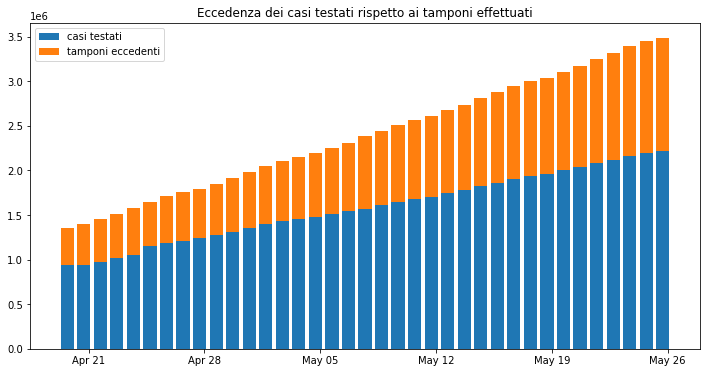
\includegraphics{tamponi.png}
            \caption{Casi testati e tamponi effettuati per COVID-19 in Italia.}
            \label{fig:tamponi}
        \end{figure}

    
    \hypertarget{introduzione}{%
\section{Introduzione}\label{introduzione}}

Recentemente i dati giornalieri pubblicati dal Dipartimento di
Protezione Civile sull'epidemia COVID-19 in Italia \cite{pcm_dpc_2020}
hanno rivelato (figura \(\ref{fig:tamponi}\)) che la quantità di casi
testati totali è attualmente solo il 64\% circa del numero di tamponi
effettuati (test RT-PCR RNA). Se ne deduce che qualche paziente è stato
sottoposto a più di un test. Perché? Quanti test sono necessari o
sufficienti per diagnosticare o escludere la patologia?

Questa breve analisi, senza pretendere di essere una trattazione
esaustiva e professionale del complesso argomento, vuole introdurre ai
concetti base per comprendere i motivi e gli strumenti matematici
sottostanti alle ripetizioni di test diagnostici qualitativi. Per
un'approfondimento più dettagliato si veda
\href{https://maxpierini.it/ncov/approfondimento-test.pdf}{Approfodimento}.

\hypertarget{test-diagnostici}{%
\section{Test diagnostici}\label{test-diagnostici}}

I test diagnostici si dividono in tre grandi categorie, in base al tipo
di risultato ottenuto \cite{porta2014dictionary}:

\begin{itemize}
\tightlist
\item
  Descrittivi
\item
  Quantitativi
\item
  Qualitativi
\end{itemize}

I risultati dei test \textbf{descrittivi} consistono perlappunto in
un'analisi descrittiva (il ``referto'', dal latino \emph{refero}) del
materiale ottenuto (il ``reperto'', dal latino \emph{repero}). È il
caso, ad esempio, di una radiografia o di un esame istologico.

I risultati dei test \textbf{quantitativi} si presentano invece come
valori numerici il cui significato, sulla base di precise linee guida
derivanti da sperimentazioni e pratica clinica, fornisce indicazioni
sullo stato di salute. Accade, ad esempio, per un emocromo o la
misurazione della pressione sanguigna.

Il risultati dei test \textbf{qualitativi} sono invece rappresentati da
un responso dicotomico, solitamente caratterizzato dalle qualità
``positivo'' \(\oplus\) o ``negativo'' \(\ominus\), che rivela la
presenza o meno di una particolare caratteristica ricercata.

I tamponi naso-faringeri utilizzati per la diagnosi di COVID-19 sono
proprio di tipo qualitativo: il risultato (ottenuto grazie all'analisi
della presenza di specifico RNA virale con metodo PCR) \(\oplus\) indica
la presenza di infezione da SARS-nCoV-2 virus e quindi di ``malattia''
\(M\) oppure la sua assenza \(\ominus\) e dunque di esclusione della
situazione patologica \(\overline{M}\) (che leggeremo ``non \(M\)'')
\cite{padhye2020reconstructed}.

Tutti i test sono caratterizzati da due importanti parametri che ne
descrivono la capacità di identificare i soggetti sani e malati
\cite{porta2014dictionary}:

\begin{itemize}
\tightlist
\item
  la \textbf{sensibilità} \(\mathbf{SE}\) è la probabilità di ottenere
  un test positivo in individui malati, ovvero \(P(\oplus|M)\) (che
  leggeremo ``probabilità di \(\oplus\) dato \(M\)'')
\item
  la \textbf{specificità} \(\mathbf{SP}\) è la probabilità di ottenere
  un test negativo in individui sani, ovvero \(P(\ominus|\overline{M})\)
  (che, similmente, leggeremo ``probabilità di \(\ominus\) dato non
  \(M\)'')
\end{itemize}

Essendo \emph{probabilità} il loro valore varia da 0 a 1 ovvero da 0\% a
100\%.

La situazione ideale sarebbe dunque di avere a disposizione un test con
\(\mathbf{SE}=1\) (100\% di test positivi su tutti i malati) e
\(\mathbf{SP}=1\) (100\% di test negativi su tutti i sani). Ma i test
diagnostici non sono strumenti perfetti e questi valori raramente sono
``tanto vicini 1'' da escludere la possibilità di errori non
trascurabili.

In particolare, falsi positivi \(F_{\oplus}\) sono i soggetti sani che
ottengono test positivi e la probabilità di ottenere un falso positivo
corrisponde pertanto alla probabilità di avere un test positivo in un
individuo sano \(P(\oplus|\overline{M})\) che, per le proprietà delle
probabilità, corrisponde al complementare della specificità

\begin{equation}\label{eq:falsipositivi}
P(F_{\oplus}) = P(\oplus|\overline{M}) = \overline{P(\ominus|\overline{M})} = 1 - P(\ominus|\overline{M}) =
1 - \mathbf{SP}
\end{equation}

Similmente, falsi negativi \(F_{\ominus}\) sono i soggetti malati che
ottengono test negativi e la probabilità di ottenere un falso negativo
corrisponde pertanto alla probabilità di avere un test negativo in un
individuo malato \(P(\ominus|M)\) che corrisponde al complementare della
sensibilità

\begin{equation}\label{eq:falsinegativi}
P(F_{\ominus}) = P(\ominus|M) = \overline{P(\oplus|M)} = 1 - P(\oplus|M) =
1 - \mathbf{SE}
\end{equation}

Pertanto (vedi figura \(\ref{fig:se-sp}\)), una bassa sensibilità
diminuisce la probabilità di avere test positivi nei malati (veri
positivi) e aumenta la probabilità di errore di ottenere test negativi
su malati (falsi negativi), mentre una bassa specificità diminuisce la
probabilità di test negativi nei sani (veri negativi) e aumenta la
probabilità di ottenere test erroneamente positivi nei sani (falsi
positivi).

Per ridurre queste probabilità di errore e migliorare \(\mathbf{SE}\) o
\(\mathbf{SP}\) di un test, laddove non ottimali, esistono diverse
strategie (consisenti nell'applicazione di più test contemporanei o
successivi in base al risultato del precedente) la cui applicazione
modifica positivamente un parametro a scapito dell'opposto. L'attenta
calibrazione di queste strategie può quindi portare a una riduzione
della probabilità degli errori non voluti senza incrementare troppo la
probabilità dell'errore opposto \cite{weinstein2005clinical}.

    \begin{figure}
\centering
    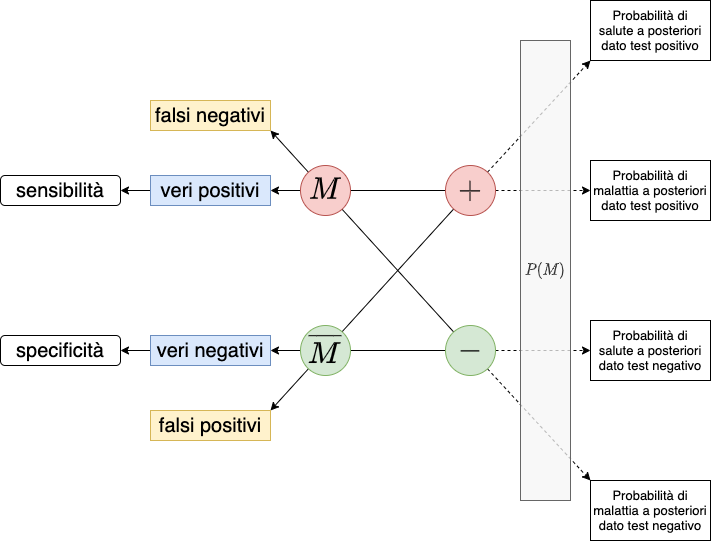
\includegraphics[width=0.5\textwidth,height=0.5\textheight,keepaspectratio]{se-sp}
    \caption{Schema di sensibilità e specificità e rapporti con le probabilità.}
    \label{fig:se-sp}
\end{figure}

    \hypertarget{probabilituxe0-di-malattia}{%
\section{Probabilità di malattia}\label{probabilituxe0-di-malattia}}

Un individuo di cui non si abbiano precedenti informazioni, estratto a
caso da una popolazione, presenta una probabilità di essere affetto da
una specifica patologia \(P(M)\) pari alla \textbf{prevalenza} della
malattia nella popolazione di riferimento. La prevalenza è misurata come
numero medio di soggetti malati nella popolazione ovvero come
percentuale di soggetti malati e dunque probabilità di estrarre un
individuo malato preso a caso dalla popolazione in oggetto.

È il caso, ad esempio, dello \emph{screening} o dei ``test a tappeto'':
non si hanno ulteriori informazioni sui soggeti se non quella di
appartenere ad una determinata popolazione (che può essere vasta come
``gli italiani'' o più ristretta come ``maschi italiani fumatori da più
di 10 anni'' o ``donne in menopausa sopra i 50 anni'') ed avere dunque
una \textbf{probabilità a priori} di malattia pari alla prevelenza della
patologia nella popolazione di appartenenza.

Nel caso invece di un paziente che presenti specifici segni, sintomi,
storia clinica precedente, fattori di rischio, risultati di precedenti
esami ecc, la sua \(P(M)\) dipende anche dalla valutazione del suo stato
e della sua anamnesi.

Nel corso di un'epidemia, la prevalenza di una particolare patologia
infettiva nella popolazione colpita, per ovvi motivi, aumenta: una
percentuale nettamente superiore di popolazione è affetta dalla malattia
ovvero la probabilità \(P(M)\) di essere malati aumenta e diminuisce di
conseguenza la probabilità di essere sani
\(P(\overline{M}) = 1 - P(M)\).

Per COVID-19 in Italia, la prevalenza in fase epidemica è stata stimata
al 13\% (circa un soggetto su 8) \cite{ceylan2020estimation}
\cite{vollmer2020sub} \cite{flaxman2020report}, ovvero un individuo
preso a caso dalla popolazione avrebbe una probabilità a priori di
essere infetto \(P(M)=13\%\) (e la quantità stimata di infetti, anche se
asintomatici, nella popolazione italiana sarebbe pari a circa
\(60'000'000 \cdot 13\% = 7'800'000\) individui!).

Sia in presenza di segni, sintomi, anamnesi caratteristica ecc, che a
prescindere da questi, l'applicazione di un test diagnostico (ad
esempio, qualitativo) incrementa o diminuisce la probabilità di malattia
\textbf{a posteriori} dell'esaminato, in particolare:

\begin{itemize}
\tightlist
\item
  \(P(M|\oplus)\) la probabilità a posteriori di malattia in seguito a
  test positivo
\item
  \(P(\overline{M}|\ominus)\) la probabilità a posteriori di salute in
  seguito a test negativo
\end{itemize}

Il \emph{Teorema di Bayes} fornisce lo strumento matematico che lega le
probabilità a posteriori di malattia dato il risultato di un test a
sensibilità e specificità del test utilizzato e alla probabilità a
priori di malattia (pari alla semplice prevalenza o alla più complessa
valutazione clinica del paziente) \cite{kruschke2014doing}.

    \hypertarget{sensibilituxe0-e-specificituxe0}{%
\section{Sensibilità e
Specificità}\label{sensibilituxe0-e-specificituxe0}}

Grazie al Teorema di Bayes sappiamo come sensibilità e specificità
modifichino la probabilità di malattia a posteriori in seguito al
risultato di un test, nota la probabilità di malattia a priori.

Tutti i tre parametri hanno effetto, positivo e negativo, sulla
probabilità di malattia a posteriori, ma in particolare:

\begin{itemize}
\tightlist
\item
  la sensibilità \(\mathbf{SE}=P(\oplus|M)\) ha maggior effetto sulla
  probabilità a posteriori di salute in seguito test negativo
  \(P(\overline{M}|\ominus)\) oltre che, come già sappiamo, sul richio
  di falsi negativi
\item
  la specificità \(\mathbf{SP}=P(\ominus|\overline{M})\) ha maggior
  effetto sulla probabilità a posteriori di malattia in seguiti a test
  positivo \(P(M|\oplus)\) oltre che, come visto in precedenza, sul
  rischio di falsi positivi
\end{itemize}

Questo significa che ad esempio, a parità di specificità, variazioni
nella sensibilità di un test produrranno una notevole variazione della
probabilità di salute se il test è negativo mentre, a parità di
sensibilità, variazioni nella specificità condurranno ad altrettanto
notevoli variazioni della probabilità di malattia in seguito a test
positivo (vedi figura \(\ref{fig:sens-spec}\)).

Per approfondimenti si veda
\href{https://maxpierini.it/ncov/approfondimento-test.pdf}{Approfodimento}.

    \begin{figure}
\centering
    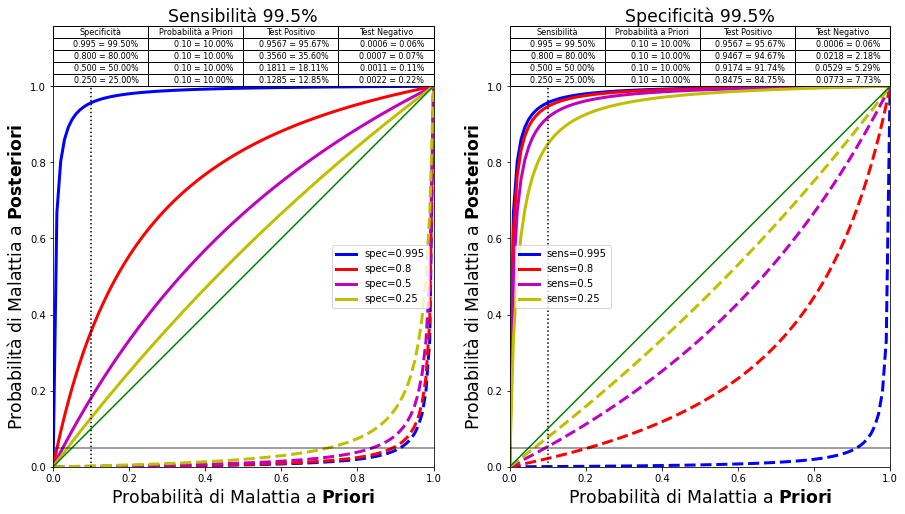
\includegraphics{sens-spec}
    \caption{Rapporto tra specificità e sensibilità. Le linee piene indicano $P(M|\oplus)$, le linee tratteggiate $P(M|\ominus).$}
    \label{fig:sens-spec}
\end{figure}

    \hypertarget{tamponi-naso-faringei-e-covid-19}{%
\section{Tamponi naso-faringei e
COVID-19}\label{tamponi-naso-faringei-e-covid-19}}

    Recenti studi suggeriscono che i test RT-PCR RNA per COVID-19 (tamponi
naso-faringei) presentino mediamente sensibilità
\(\mathbf{SE} = 0.777 = 77.70\%\) e specificità
\(\mathbf{SP}=0.988=98.80\%\) \cite{padhye2020reconstructed}.

    
    Ci troviamo dunque di fronte ad un test piuttosto specifico che
comporterà una probabilità relativamente esigua di falsi positivi

    \[
P(F_{\oplus}) = 1 - P(\ominus|\overline{M}) = 1 - \mathbf{SP} = 1 - 0.988 = 0.012 = 1.20\%
\]

    
    e ad una notevole variazione della probabilità di malattia a posteriori
in seguito a risultato positivo.

Ma, al contempo, il test non ha una sensibilità ottimale e il rischio di
falsi negativi è decisamente più elevato

    \[
P(F_{\ominus}) = 1 - P(\oplus|M) = 1 - \mathbf{SE} = 1 - 0.777 = 0.223 = 22.30\%
\]

    
    così come si ottiene una minore variazione nella probabilità di salute a
posteriori in seguito a risultato negativo.

L'applicazione di una delle strategie a cui abbiamo accennato può però
migliorare la scarsa sensibilità senza ``degradare'' eccessivamente
l'accettabile specificità.

    \hypertarget{test-ripetuti}{%
\section{Test ripetuti}\label{test-ripetuti}}

A prescindere dall'utilizzo di esami differenti (come radiografie e test
sierologici) e dalla rivalutazione clinica delle condizioni del
paziente, l'applicazione della strategia nota come \textbf{Regola O
serial} (the OR rule in serial tests) è volta propriamente ad aumentare
la sensibilità di un test (a scapito della specificità):

\begin{itemize}
\tightlist
\item
  il test viene ripetuto \(n\) volte solo se precedentemente negativo
\item
  è sufficiente che uno solo dei test risulti positivo per confermare la
  situazione patologica
\item
  solo se tutti gli \(n\) test sono negativi è eclusa la malattia.
\end{itemize}

Data la prevalenza stimata di COVID-19 in Italia e la necessità di
dosare attentamente il numero di tamponi effettuati vista la loro
scarsità, si rende necessario applicare la regola di ripetizione (vedi
figura \(\ref{fig:ripetizione-covid}\)) solo in particolari casi come
soggetti a rischio notevolmente elevato, precedenti ospedalizzati
dimessi, pazienti con segni e sintomi rilevanti, ecc che aumentino la
probabilità di malattia a posteriori in maniera decisiva rispetto alla
semplice prevalenza (vedi figura \(\ref{fig:covid}\)).

    È infatti sufficiente un solo test negativo in un soggetto con
probabilità di malattia a priori pari alla sola prevalenza
\(P(M)=13.00\)\% per portare la probabilità di salute a posteriori in
seguito a test negativo, al di sopra di una soglia accettabile
\(P(\overline{M}|\ominus) = 96.74\)\%

    
    Al comtempo, è sufficiente un solo test positivo in un soggetto con
probabilità di malattia a priori pari alla sola prevalenza per aumentare
notevolmente la probabilità di malattia a posteriori in seguito a test
positivo \(P(M|\oplus) = 90.63\)\%

    
    Assumendo per semplicità quest'ultima come nuova probabilità a priori di
malattia in un soggetto precedentemente diagnosticato come malato, ad
elevato rischio o con segni e sintomi caratteristici, effettuando un
test per verificare che sia sano o guarito e presumendo che risulti
negativo, la sua probabilità di salute a posteriori non è più
accettabile, avrebbe infatti \(P(\overline{M}|\ominus) = 31.41\%\) e
quindi ancora una probabilità di essere malato notevolmente elevata
\(P(M|\ominus) = 1 - P(\overline{M}|\ominus) = 68.59\%\)

    
    A prescindere quindi (come si diceva) dalla valutazione clinica e/o da
altri esami effettuati, dato che il test è risultato negativo, si può
procedere con la \textbf{Regola O} sottoponendolo ad un nuovo tampone.
Come accennato però, le strategie di ripetizione modificano sia
sensibilità che specificità e (applicando le formule corrispondenti)
otterremo un test con

\[
\mathbf{SE}_2 = 1 - (1 - \mathbf{SE})^2 = 1 - (1 - 0.777)^2 = 0.9503 = 95.03\%
\]

\[
\mathbf{SP}_2 = \mathbf{SP}^2 = 0.988^2 = 0.9761 = 97.61\%
\]

    
    \begin{figure}
\centering
    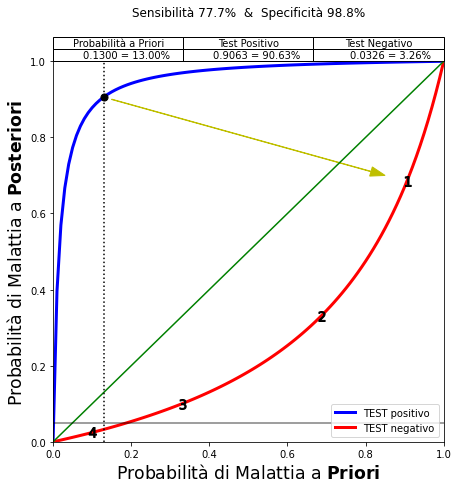
\includegraphics[width=0.5\textwidth,height=0.5\textheight,keepaspectratio]{covid}
    \caption{Probabilità di malattia COVID-19 a posteriori per test RT-PCR SARS-CoV-2 RNA con ripetezione seriale dei test Regola $\mathbf{O}$}
    \label{fig:covid}
\end{figure}

    Abbiamo pertanto incrementato la sensibilità del 17.33\% a scapito di
una diminuzione della specificità pari al -1.19\%.

Sulla base di questi nuovi parametri effettuiamo un nuovo test assumendo
come probabilità di malattia a priori il risultato ottenuto dal test
precedente \(P(M)=68.59\)\%

\[
P(M|\oplus) = 98.86\%
\]

\[
P(\overline{M}|\ominus) = 89.99\%
\]

    
    Notiamo che effettivamente un risultato positivo confermerebbe la
diagnosi di malattia (e il falso negativo del test precedente) ma se il
test risultasse negativo, nonostante la probabilità di salute sia molto
più elevata rispetto al test precedente, otterremmo comunque una
probabilità di malattia a posteriori non ottimale per escludere la
patologia \(P(M|\ominus) = 1 - P(\overline{M}|\ominus) = 10.01\)\% dato
anche il rischio di contagio in corso di epidemia.

    
    Perciò, se il test fosse risultato negativo, applicando nuovamente la
\textbf{Regola O} potremmo sottoporre il soggetto ad un nuovo tampone,
sapendo però che influirà ancora su sensibilità e specificità

\[
\mathbf{SE}_3 = 1 - (1 - \mathbf{SE})^3 = 1 - (1 - 0.777)^3 = 0.9889 = 98.89\%
\]

\[
\mathbf{SP}_3 = \mathbf{SP}^3 = 0.988^3 = 0.9644 = 96.44\%
\]

    
    Otterremo dunque un incremento totale della sensibilità del 21.19\% a
scapito di una diminuzione complessiva della specificità del -2.36\%.

Effettuiamo il terzo test coi nuovi parametri e assumendo come
probabilità di malattia a priori il risultato ottenuto dal secondo test
negativo \(P(M)=10.01\)\%

\[
P(M|\oplus) = 75.57\%
\]

\[
P(\overline{M}|\ominus) = 99.87\%
\]

    
    Siamo giunti pertanto, grazie alle regole di ripetizione dei test
diagnostici, ad ottenere una probabilità di malattia a posteriori del
terzo tampone negativo pari ad un esiguo \(P(M|\ominus)=0.13\)\% ma al
contempo avremmo una probabilità di malattia in caso di test positivo
sufficiente a ritenere il paziente non guarito o comunque molto
probabilmente infetto e attuare le necessarie azioni successive
(isolamento, ospedalizzazione, altri esami, terapie, ecc) a seconda
delle condizioni generali del paziente, dei suoi fattori di rischio, ecc
\cite{centers2020interim} \cite{bai2020presumed}
\cite{national2020coronavirus}.

    
    \begin{figure}
\centering
    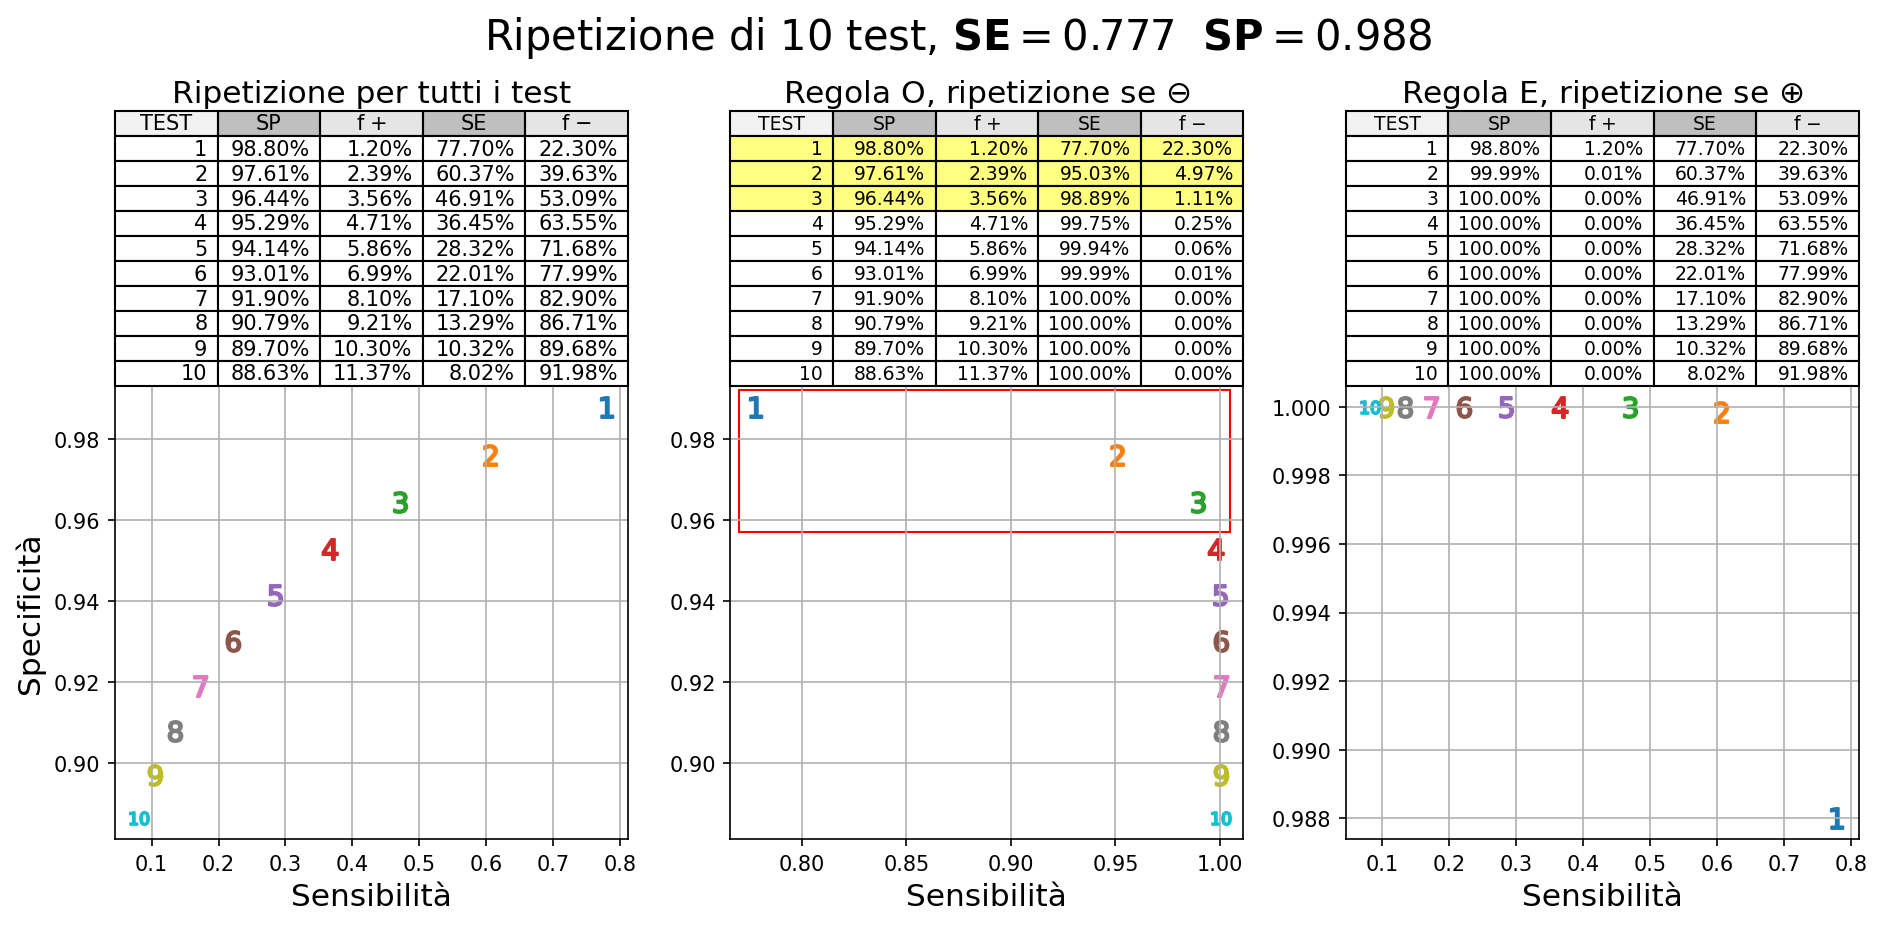
\includegraphics{ripetizione-covid}
    \caption{Effetto delle regole di ripetizione sui test RT-PCR per COVID-19}
    \label{fig:ripetizione-covid}
\end{figure}

    \hypertarget{conclusioni}{%
\section{Conclusioni}\label{conclusioni}}

Grazie alle proprietà matematiche di sensibilità, specificità,
probabilità di malattia a priori e a posteriori e regole di ripetizione
dei test diagnostici qualitativi, si può giungere al miglioramento della
non ottimale sensibilità dei tamponi naso-faringei utilizzati nella
diagnosi di COVID-19, diminuendo il rischio di falsi negativi e
ottenendo un'accettabile probabilità di salute in seguito a test
negativo dopo il terzo tampone ripetuto con Regola \textbf{O} (solo se
negativo) senza rischiare un'eccessiva diminuzione della buona
specificità iniziale e mantenendo dunque una probabilità accettabile di
falsi positivi e di malattia a seguito di test positivo. L'analisi
spiega pertanto, vista l'importanza dei falsi negativi per il
contenimento di un'evento epidemico, la discrepanza tra tamponi
effettuati e casi totali testati nel corso dell'attuale epidemia di
COVID-19 in Italia.


    % Add a bibliography block to the postdoc
    
    
\bibliographystyle{IEEEtran}
\bibliography{IEEEabrv,biblio}

    
\end{document}
